
\documentclass[10pt]{beamer}

\mode<presentation> {

\usetheme{CambridgeUS}
\usecolortheme{dolphin}
\setbeamertemplate{footline}[frame number] % To replace the footer line in all slides with a simple slide count uncomment this line
\setbeamertemplate{navigation symbols}{} % To remove the navigation symbols from the bottom of all slides uncomment this line
}


\usepackage{graphicx} % Allows including images
\usepackage{subcaption}
\usepackage{booktabs} % Allows the use of \toprule, \midrule and \bottomrule in tables
\usepackage{wrapfig}
\usepackage{multirow}
\usepackage{lipsum}
\usepackage{xcolor}
\usepackage{amsmath,amssymb}
\usepackage{array}
\usepackage{animate,media9,movie15}
\usepackage[english]{babel}
\usepackage{ragged2e}
\usepackage{amssymb,amsfonts,amsmath}
\usepackage{tikz,tkz-euclide}
\usepackage{appendixnumberbeamer}
\usefonttheme[]{serif}

%----------------------------------------------------------------------------------------
%	TITLE PAGE                                                                           |
%----------------------------------------------------------------------------------------

\title[]{ROS-Based \textbf{M}ulti-\textbf{A}gent \textbf{S}ystems \textbf{CO}ntrol Simulation \textbf{T}estbed (MASCOT)} % The short title appears at the bottom of every slide, the full title is only on the title page

\author[]{Arvind Pandit, Akash Njattuvetty, and Ameer K. Mulla} % Your name
\titlegraphic{
	
\includegraphics[origin=c,scale=0.30]{icc_l.png}\qquad\qquad
\includegraphics[scale=0.05]{IITDh_Logo.png}
}

\institute[] % Your institution as it will appear on the bottom of every slide, may be shorthand to save space
{
	Department of Electrical Engineering\\
	Indian Institute of Technology Dharwad, India
	%\medskip
}
\date{Indian Control Conference (ICC-8) \\ 14-16 December 2022, Chennai, India.}

\begin{document}


\begin{frame}[plain,noframenumbering]
	%[noframenumbering]
	\titlepage % Print the title page as the first slide
	%	\begin{figure}
	%		\centering \includegraphics[scale=cale=0.5]{IITDh_Emblem.jpg}
	%	\end{figure}
\end{frame}

\begin{frame}
	\frametitle{Overview} % Table of contents slide, comment this block out to remove it
	\tableofcontents % Throughout your presentation, if you choose to use \section{} and \subsection{} commands, these will automatically be printed on this slide as an overview of your presentation
\end{frame}

%----------------------------------------------------------------------------------------
%	PRESENTATION SLIDES
%----------------------------------------------------------------------------------------

%----------------------------------------------------------

\section*{}
\begin{frame}{}
	\huge{\centerline{\textcolor{blue}{\textbf{Multi-Agent Systems}}}}
\end{frame}

\section{Introduction}
\subsection*{Multi-Agent Systems}

%----------------------------------------------------------
\begin{frame}
	\frametitle{Multi-Agent Systems}

	\begin{block}{\textbf{Multi-Agent Systems:}}
		\justifying  A system consists of multiple co-operative agents interacting with each other.
		\vspace*{0.1 cm}
	\end{block}

	\begin{block}{\textbf{Distributed Control:}}

		\begin{itemize}
			\item Control is distributed among multiple agents.
			\item Each agent with it's own local control algorithm.
			\item Communicating with each other.
		\end{itemize}
		\vspace*{0.1 cm}
	\end{block}
	\pause
	\begin{block}{\textbf{Advantages:}}

		\begin{itemize}
			\item Achieve complex objectives.
			\item Faster exploration.
		\end{itemize}
		\vspace*{0.1 cm}
	\end{block}
	\pause
	\begin{block}{\textbf{Applications:}}
		Robotics, space missions, search and exploration, surveillance, agriculture etc.
	\end{block}



\end{frame}
%----------------------------------------------------------.
\subsection*{Simulation Platform for Multiagent System}

\begin{frame}
	\frametitle{Simulation Platform for Multiagent System}
	\begin{block}{\textbf{Simulation:}}
		\begin{itemize}
			\item Test the performance of robot before it is built.
			\item Evaluate different control laws.
			\item Train in safe and controlled environment.
			\item Study the behaviour of the system.
		\end{itemize}
		\pause
		\vspace*{0.1 cm}
	\end{block}
	\begin{block}{\textbf{Existing MAS Simulation:}}
		\begin{itemize}
			\item MATLAB based simulators.
			\item Limitation of no. of agents.
			\item Not readily deployable of hardware.
		\end{itemize}
	\end{block}

\end{frame}


\subsection*{MASCOT}


\begin{frame}
	\frametitle{MASCOT}
	\begin{itemize}
		\item Developed using open source tools.
		\item ROS and Gazebo.
		\item Supports low level driver.
		\item Simple user interface.
		\item In this version Quadcopter as an agent.
		\item Multiagent system with double integrator.
		\item Easy to setup with Docker Support.
	\end{itemize}
	\vspace*{0.2 cm}
	\pause
	\begin{minipage}{0.47\textwidth}
		\begin{figure}[h!]
			\centering
			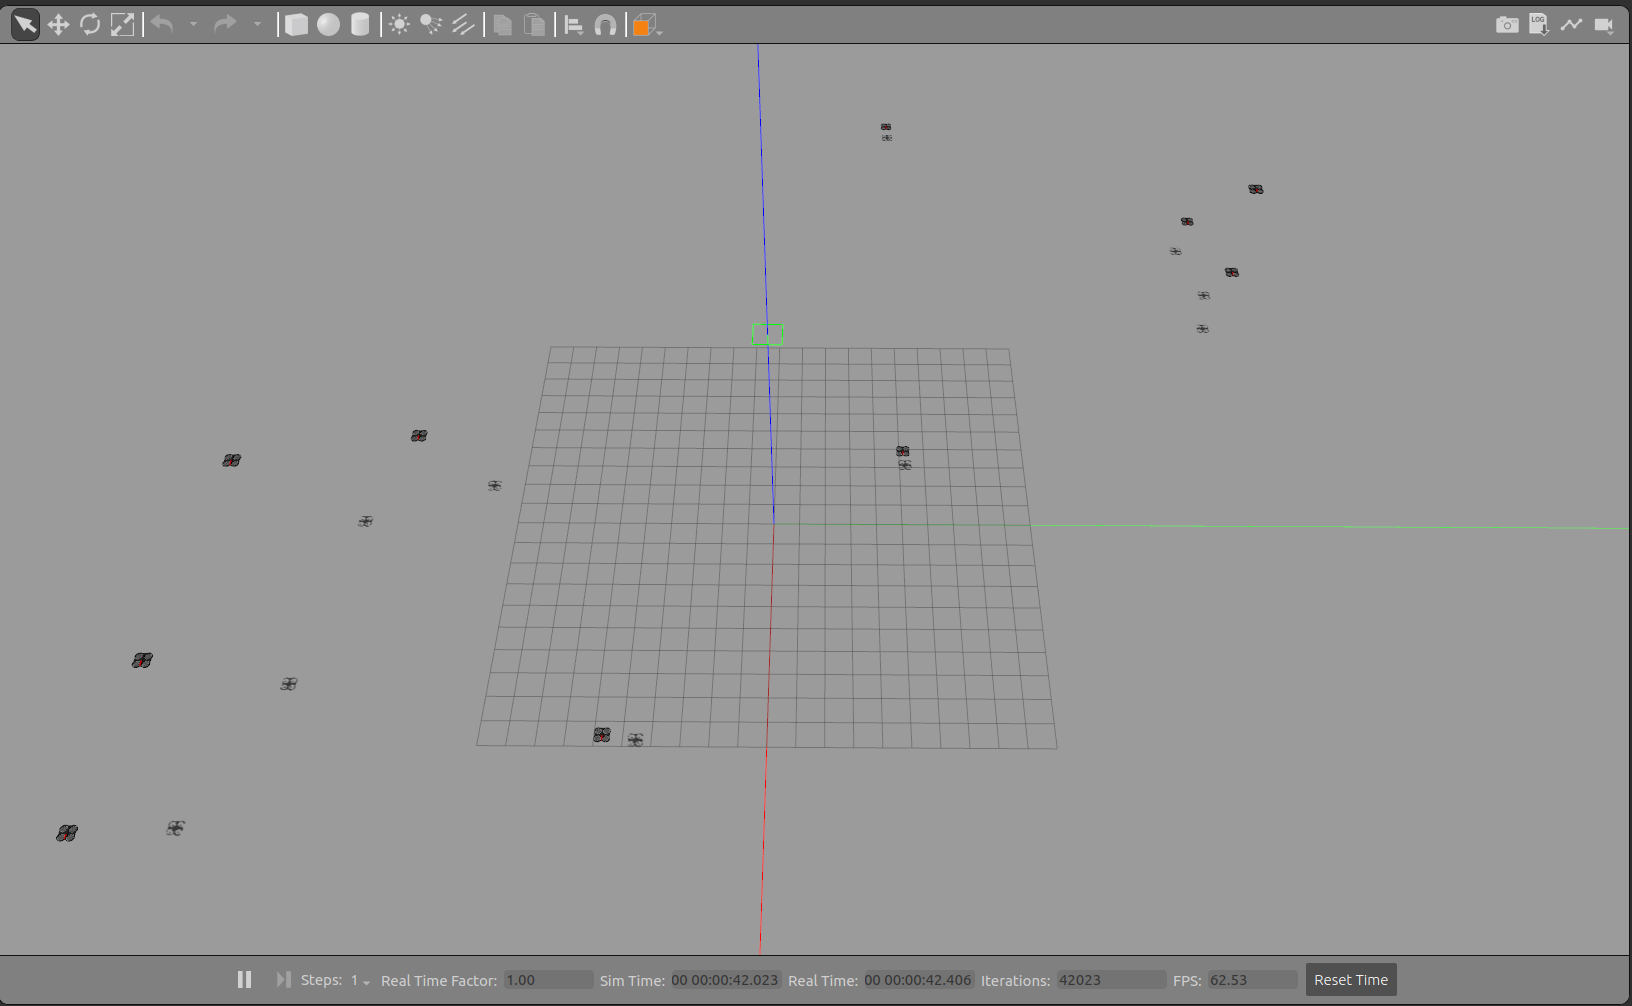
\includegraphics[scale=0.09]{10-drone-position-not-aligned.png}
			\caption{Initial Position of Drones}
			\label{Fig:pos_in}
		\end{figure}
	\end{minipage}
	\begin{minipage}{0.47\textwidth}
		\begin{figure}[h!]
			\centering
			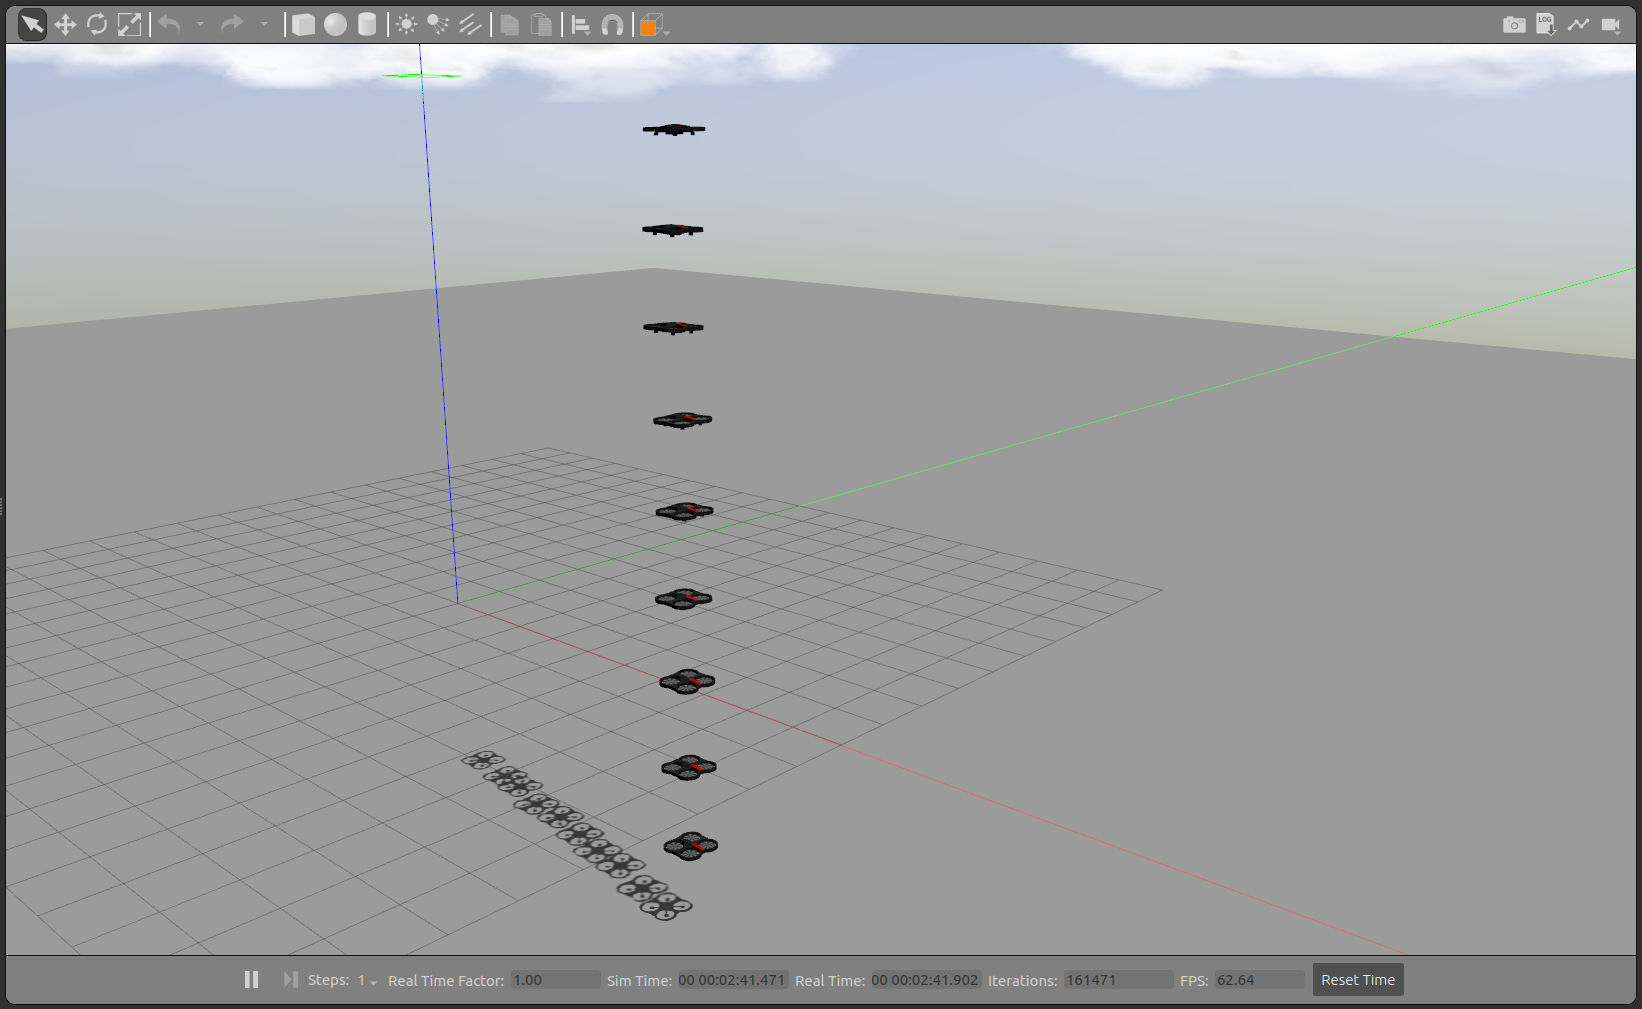
\includegraphics[scale=0.09]{10-drone-position-aligned.png}
			\caption{Final Position}
			\label{Fig:pos_fi}
		\end{figure}
	\end{minipage}

\end{frame}
%------------------------------------------------------------.

\section*{}
\begin{frame}{}
	\huge{\centerline{\textcolor{blue}{\textbf{Preliminaries}}}}
\end{frame}
\section{Preliminaries}
%------------------------------------------------------------
\subsection*{Frame of Reference}
%-----------------------------------------------------------/
\begin{frame}
	\frametitle{Frame of Reference\footnote{P. I. Corke \textit{et al.},Robotics, vision and control: fundamental algorithms in MATLAB}}
	\begin{figure}[h!]
		\centering
		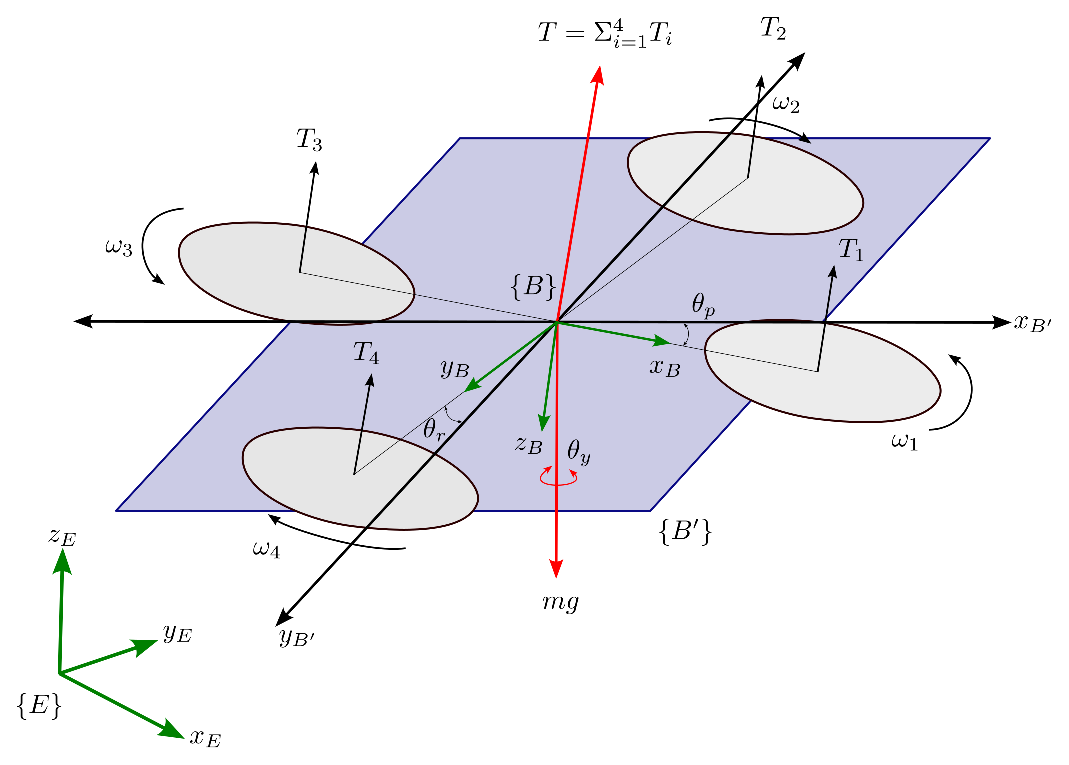
\includegraphics[scale=0.5]{Quadcopter.eps}
		\caption{Frame of Reference}
		\label{Fig:Frame_of_Reference.}
	\end{figure}
\end{frame}
%%-----------------------------------------------------------
%%-----------------------------------------------------------
\subsection*{Quadcopter Dynamics}
%------------------------------------------------------------
\begin{frame}
	\frametitle{Quadcopter Dynamics}
	\begin{itemize}
		\item The total upward thrust along the $-z^{B}$ axis is given by
		      \begin{equation}
			      \mathbf{T} = \Sigma (b {\omega}_{i}^2)
		      \end{equation}
		\pause
		\vspace*{-0.4 cm}
		\item The translation dynamics of the quadcopter in $\{E\}$ is
		      \begin{equation}
			      m\dot{\mathbf{v}}^{E}=\begin{bmatrix}
				      0 & 0 & m g
			      \end{bmatrix}^{T}-\mathbf{R}_{B}^{E}\begin{bmatrix}
				      0 & 0 & T
			      \end{bmatrix}^{T} - B\mathbf{v}\label{eq:trans_dynamics}
		      \end{equation}
			  \pause
			  \vspace*{-0.4 cm}
		\item Torque about $x$ and $y$ axes is
		      \begin{equation}
			      \tau_{x}=d T_{4}-d T_{2} = db(\bar{\omega}_{4}^{2}-\bar{\omega}_{2}^{2})
		      \end{equation}
		      \begin{equation}
			      \tau_{y}=d T_{1}-d T_{3} = db(\bar{\omega}_{1}^{2}-\bar{\omega}_{3}^{2})
		      \end{equation}
			  \pause
			  \vspace*{-0.4 cm}
		\item The total reaction torque about $z$-axis is
		      \begin{equation}
			      \tau_{z} =Q_{1}-Q_{2}+Q_{3}-Q_{4}=k\left(\bar{\omega}_{1}^{2}+\bar{\omega}_{3}^{2}-\bar{\omega}_{2}^{2}-\bar{\omega}_{4}^{2}\right)\label{eq:react_torque_z}
		      \end{equation}
			  \pause
			  \vspace*{-0.4 cm}
		\item By Euler's equation of motion rotational acceleration is
		      \begin{equation}
			      J\boldsymbol{\Dot{\omega}}=-\boldsymbol{\omega} \boldsymbol{\times}J \boldsymbol{\omega}+\mathbf{\Gamma}
		      \end{equation}
			  \pause
			  \vspace*{-0.4 cm}
		\item Overall quadcopter motion equation
		      \begin{align}
			      \begin{bmatrix}
				      \mathbf{T} &
				      \mathbf{\Gamma}
			      \end{bmatrix}^T & =A\begin{bmatrix}
				      \bar{\omega}_{1}^{2} &
				      \bar{\omega}_{2}^{2} &
				      \bar{\omega}_{3}^{2} &
				      \bar{\omega}_{4}^{2}
			      \end{bmatrix}^T
		      \end{align}

	\end{itemize}

\end{frame}
%%--------------------------------.
%%----------------------------------------------------------
\subsection*{Quadcopter Dynamics as Double Integrator}
%-----------------------------------------------------------
\begin{frame}{Quadcopter Dynamics as Double Integrator}
	\begin{minipage}{0.47\textwidth}
		\begin{itemize}
			\item Total force on quadcopter
			      \begin{equation*}
				      \mathbf{f}^{B^{\prime}}=\mathbf{R}{x}\left(\theta{r}\right) \mathbf{R}{y}\left(\theta{p}\right)\begin{bmatrix}
					      0 & 0 & T
				      \end{bmatrix}^{T}\label{eq:total_force}
			      \end{equation*}

			\item Thus we get $\mathbf{f}^{B^{\prime}}$ as
			      \begin{equation*}
				      \mathbf{f}^{B^{\prime}}=\begin{bmatrix}
					      T\sin{\theta_{p}}                 \\
					      T\sin{\theta_{r}}\cos{\theta_{p}} \\
					      T\cos{\theta_{r}}\cos{\theta_{p}}
				      \end{bmatrix}
			      \end{equation*}
		\end{itemize}
	\end{minipage}
	\begin{minipage}{0.47\textwidth}
		\begin{figure}[h!]
			\centering
			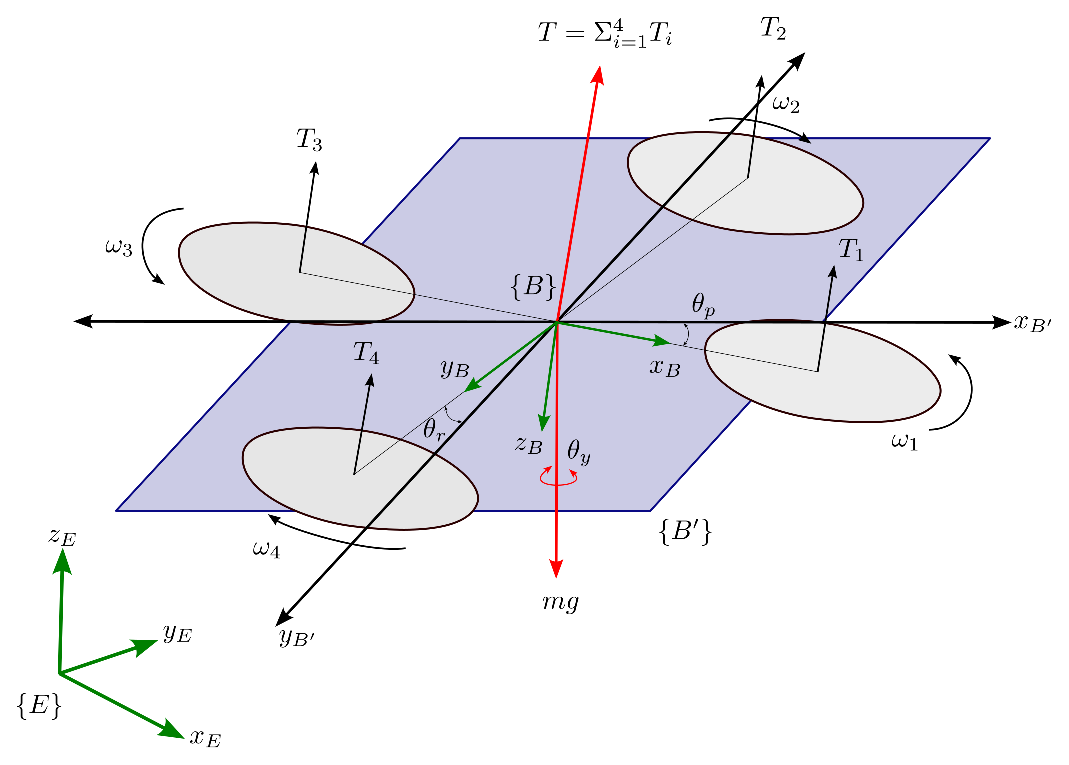
\includegraphics[scale=0.28]{Quadcopter.eps}
			\caption{Quadcopter Dynamics}
			\label{Fig:Quadcopter Dynamics}
		\end{figure}
	\end{minipage}
	\pause
	\begin{itemize}
		\item For small $\theta_{p}$ and $\theta_{r}$ the $\mathbf{f}^{B^{\prime}}$ can be approximated by
		      \begin{equation*}
			      \mathbf{f}^{B^{\prime}} \approx \begin{bmatrix}
				      T\theta_{p} & T\theta_{r} & T
			      \end{bmatrix}^{T}
		      \end{equation*}
		\item With this assumption the Quadcopter can be assumed as a double integrator system where $\theta_{p}$ and $\theta_{r}$ are given by
		      \begin{equation*}
			      \theta_{p} = \dfrac{m}{T}a_{x}^{B^{\prime}},~~\theta_{r} = \dfrac{m}{T}a_{y}^{B^{\prime}}
		      \end{equation*}
	\end{itemize}
\end{frame}
%%---------------------------------------------------------
\section*{}
\begin{frame}{}
	\huge{\centerline{\textcolor{blue}{\textbf{MASCOT:Structure and Features}}}}
\end{frame}

\section{MASCOT:Structure and Features}

\subsection*{Tools Used}
%----------------------------------------------------------
\begin{frame}
	\frametitle{Tools Used}
	\begin{block}{\textbf{ROS:}}
		\begin{itemize}
			\item Open source robotics framework.
			\item Distributed architecture with intercommunication between different nodes.
			\item Support for various programming language Python, C++, Java.
			\item Rich visualization and debugging tools.
		\end{itemize}
	\end{block}
	\pause
	\begin{block}{\textbf{Gazebo:}}
		\begin{itemize}
			\item 3D simulation platform.
			\item Uses Open Dynamics Engine for realtime physics simulation.
			\item Support for sensor and actuator plugin.
		\end{itemize}
	\end{block}
	\pause
	\begin{block}{\textbf{TUM Simulator Package:}}
		\begin{itemize}
			\item Uses the AR Parrot drone model.
			\item Low level plugin is modified as per the Double integrator dynamics.
			\item Added the required topics and controls.
		\end{itemize}
	\end{block}
\end{frame}
%--------------------------------------------------------------
\subsection*{Control Block}
\begin{frame}
	\frametitle{Control Block}
	\begin{figure}[h!]
		\centering
		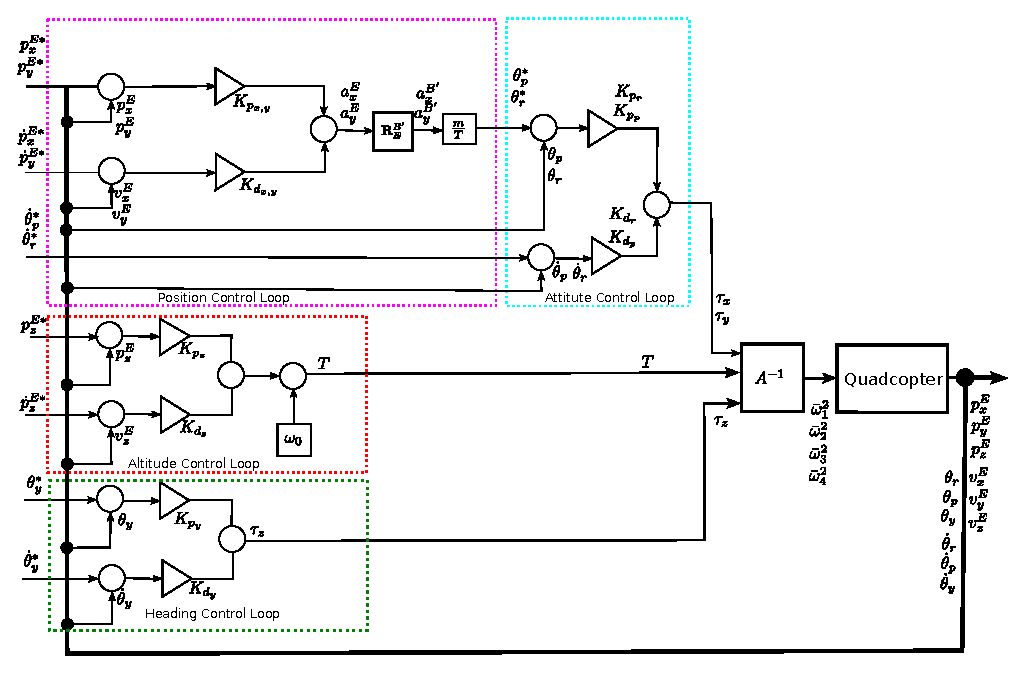
\includegraphics[scale=0.6]{Control-block.eps}
		\caption{Control Block}
		\label{Fig:Control Block}
	\end{figure}
\end{frame}

\subsection*{Architecture}
\begin{frame}
	\frametitle{Architecture}
	\begin{figure}[h!]
		\centering
		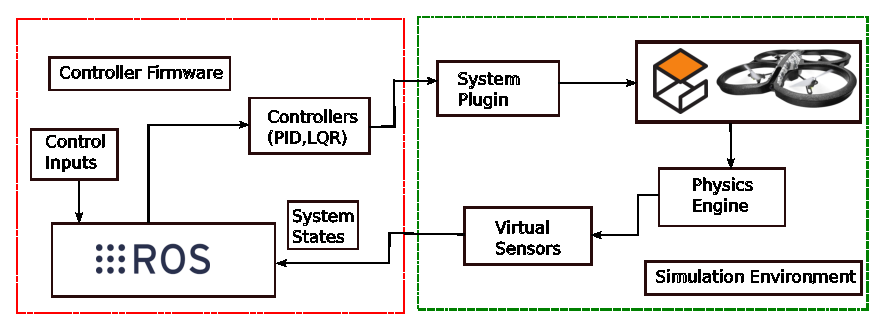
\includegraphics[scale=0.8]{System-architecture.eps}
		\caption{System Architecture}
		\label{Fig:System Architecture}
	\end{figure}
	\begin{itemize}
		\item Gazebo internal scheduler provides the ROS interface.
		\item ROS works as middleware which runs independent controller for each agent.
		\item The intercommunication uses TCPROS protocol.
	\end{itemize}
\end{frame}

\subsection*{Feature and Configuration of Simulation Testbed}
\begin{frame}{Feature and Configuration of Simulation Testbed}
	\vspace*{-0.2 cm}
	\begin{block}{Feature}
		\begin{itemize}
			\item Easy modification.
			\item Supports multiple languages Python, Cpp, Java.
			\item Flexibility with no. of agents.
		\end{itemize}
	\end{block}
	\pause
	\vspace*{-0.2 cm}
	\begin{block}{Configuration}
	\begin{minipage}{0.47\textwidth}
		\begin{itemize}
			\item \textbf{Robot:} Details of the Robots to be simulated
			      \begin{itemize}
				      \item \textbf{Number:} No. of Agents.
				      \item \textbf{IntialPosition:} Enable initializer.
				      \item \textbf{Position:} Initial Position.
			      \end{itemize}
			\item \textbf{Output:} Output config
			      \begin{itemize}
				      \item \textbf{Velocity : }Generate Vel plot.
				      \item \textbf{Position : }Generate Vel plot.
				      \item \textbf{Save-plot : }Save plots.
				      \item \textbf{Show-plot : }Show plots.
				      \item \textbf{Save-data : }Save Numpy array.
			      \end{itemize}
		\end{itemize}
	\end{minipage}
	\begin{minipage}{0.47\textwidth}
		\begin{itemize}
			\item \textbf{Control: }Controls laws
			      \begin{itemize}
				      \item \textbf{Custom-Control: }
				      \item \textbf{Tutorial Examples: }
				      \item[*] \textbf{Waypoint Navigation:}
				            \begin{itemize}
					            \item[-] \textbf{P-Gain: }Default = 1.0
					            \item[-] \textbf{D-Gain: }Default = 1.0
				            \end{itemize}
				      \item[*] \textbf{Consensus: }
				            \begin{itemize}
					            \item[-] \textbf{Leader: }Robot index to be leader, 0-for leaderless.
					            \item[-] \textbf{Communication Graph: }
					            \item[-] \textbf{L-mat: } Laplacian Matrix.
				            \end{itemize}
				      \item[*] \textbf{Min-max Consensus: }
			      \end{itemize}
		\end{itemize}
	\end{minipage}		
\end{block}
\end{frame}

%-----------------------------------------------------
\section*{}
\begin{frame}{}
	\huge{\centerline{\textcolor{blue}{\textbf{Examples}}}}
\end{frame}
\section{Examples}
%-----------------------------------------------------

\subsection*{Way-Point Navigation}
\begin{frame}
	\begin{itemize}
		\item  The position of the quadcopter in $x^{B^{\prime}}y^{B^{\prime}}$ plane is controlled independently by  the proportional-derivative controller for each axis.
		      \begin{equation*}\label{x-pos-control}
			      a_{x} = K_{p_{x}}\left(p_{x}^{*}-p_{x}\right)+K_{d_{x}}\left(\dot{p}_{x}^{*}-\dot{p}{x}\right)
		      \end{equation*}
		      \begin{equation*}\label{y-pos-control}
			      a_{y} = K_{p_{y}}\left(p_{y}^{*}-p_{y}\right)+K_{d_{y}}\left(\dot{p}_{y}^{*}-\dot{p}{y}\right)
		      \end{equation*}
	\end{itemize}
	\pause
	\frametitle{Way-Point Navigation}
	\begin{minipage}{0.47\textwidth}
		\begin{figure}[h!]
			\centering
			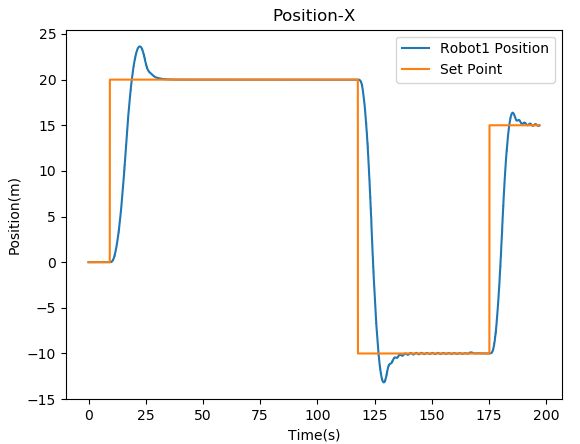
\includegraphics[scale=0.27]{Position-X-single.png}
			\caption{X-axis Position plot of Waypoint Navigation}
			\label{Fig:pos_x}
		\end{figure}
	\end{minipage}
	\begin{minipage}{0.47\textwidth}
		\begin{figure}[h!]
			\centering
			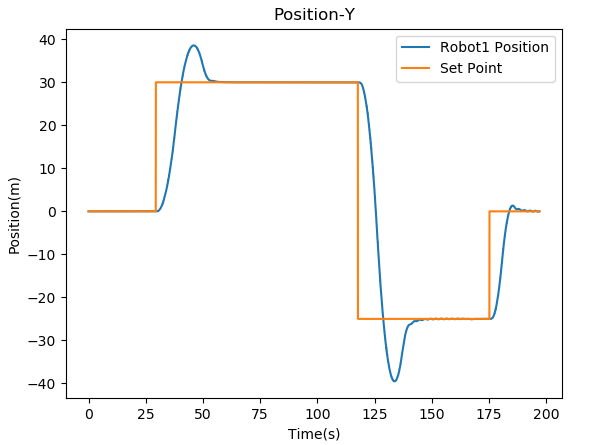
\includegraphics[scale=0.27]{Position-Y-single.png}
			\caption{Y-axis Position plot of Waypoint Navigation}
			\label{Fig:pos_y}
		\end{figure}
	\end{minipage}
\end{frame}

\subsection*{Consensus Algorithm (Linear)}
\begin{frame}
	\frametitle{Consensus Algorithm (Linear)}
	\begin{itemize}
		\item A leaderless asymptotic consensus and leader follower is implemented.
		\item The control algorithms used is as follows:\footnote{A.Joshi\textit{ et al.} Implementation of distributed consensus on an outdoor testbed,2016 ECC}
		      \begin{equation*}
			      \textbf{f}_{i}^{E}=\left\{\begin{array}{l}
				      \sum_{j = 1}^{n} a_{ij}\left(\mathbf{p}{j}^{E}-\mathbf{p}{i}^{E}\right)-\beta \textbf{v}_{i}^{E} \text { if } \alpha_{i} \in \mathbf{F} \\
				      \\
				      0 \text { if }  \alpha_{i} \in \mathbf{L}
			      \end{array}\right.
		      \end{equation*}
	\end{itemize}
	\pause
	\begin{minipage}{0.47\textwidth}
		\begin{figure}[h!]
			\centering
			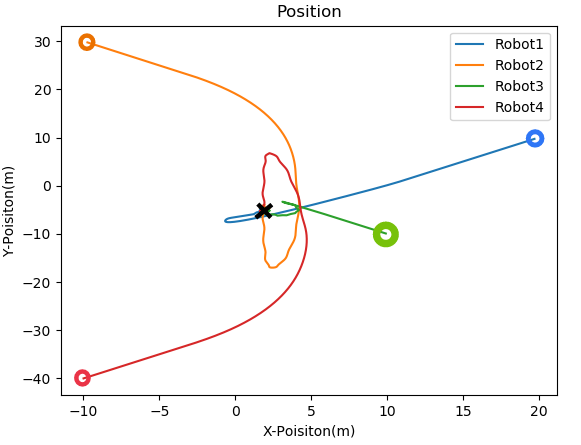
\includegraphics[scale=0.27]{Position.png}
			\caption{Leaderless Control plot}
			\label{Fig:pos_x_c}
		\end{figure}
	\end{minipage}
	\begin{minipage}{0.47\textwidth}
		\begin{figure}[h!]
			\centering
			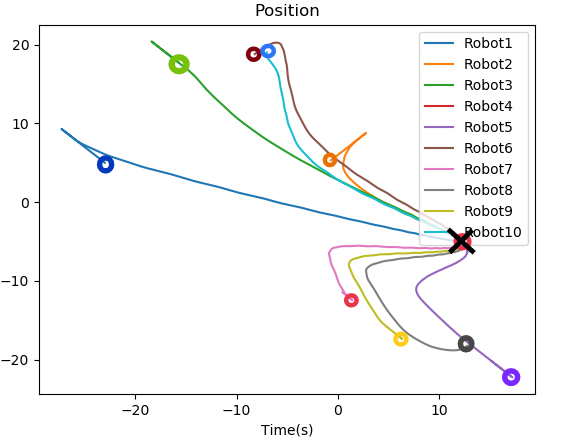
\includegraphics[scale=0.27]{Position-leader.png}
			\caption{Leader Follower plot}
			\label{Fig:pos_y_c}
		\end{figure}
	\end{minipage}


\end{frame}

\subsection*{Min-Max Time Consensus}
\begin{frame}
	\frametitle{Min-Max Time Consensus}
	\begin{itemize}
		\item A non linear Min-Max time consensus Algorithm is implemented.
		\item The Control Law used is \footnote{A. Joshi\textit{ et al.} Implementation of min-max time consensus tracking on a multi-quadrotor testbed,2019 ECC}
		      \begin{equation*}
			      \mathbf{f}^E_c=\beta_c\text{sign}(2(\beta_c-\beta_p)(\mathbf{p}_c-\mathbf{p}_p)+(\mathbf{v}_c-\mathbf{v}_p)^2\text{sign}(\mathbf{v}_c-\mathbf{v}_p))
		      \end{equation*}
	\end{itemize}
	\pause
	\begin{minipage}{0.47\textwidth}
		\begin{figure}[h!]
			\centering
			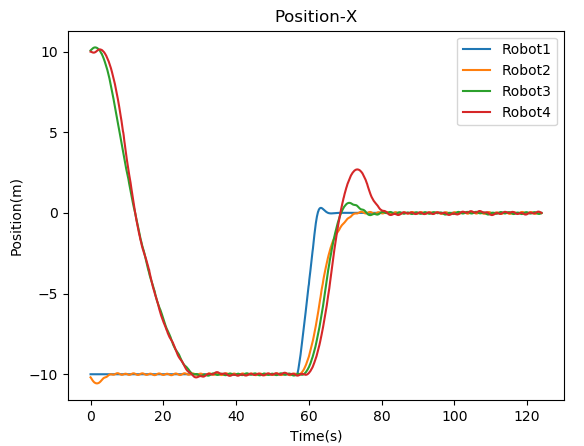
\includegraphics[scale=0.27]{Position-X-minmax.png}
			\caption{Position in X axis}
			\label{Fig:pos_x_m}
		\end{figure}
	\end{minipage}
	\begin{minipage}{0.47\textwidth}
		\begin{figure}[h!]
			\centering
			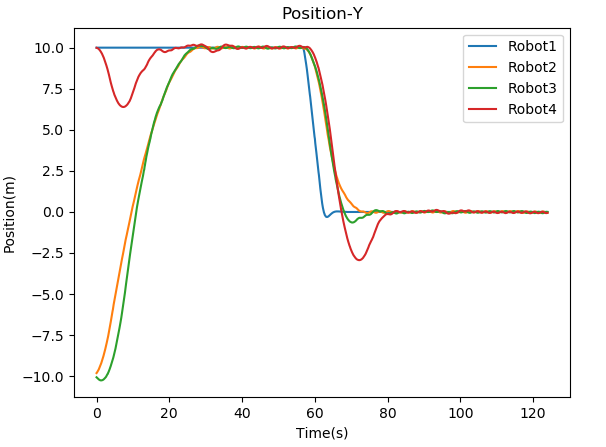
\includegraphics[scale=0.27]{Position-Y-minmax.png}
			\caption{Position in Y axis}
			\label{Fig:pos_y_m}
		\end{figure}
	\end{minipage}
\end{frame}


\section*{}
\begin{frame}{}
	\huge{\centerline{\textcolor{blue}{\textbf{Conclusion and Future Work}}}}
\end{frame}

\section{Conclusion and Future Work}
\begin{frame}{Conclusion and Future Work}
	\begin{block}{Conclusion}
		\begin{itemize}
			\item A simulation testbed for MultiAgent System.
			\item Quadcopter are approximated as a double integrator system.
			\item Various Linear and Non-Linear control laws are tested.
			\item This shows the integrity of the developed testbed.
		\end{itemize}
	\end{block}

	\pause \begin{block}{Future Work}
		\begin{itemize}
			\item System is Open-source and expandable.
			\item UGVs and different UAVs can be deployed.
			\item Human In the loop control.
			\item Deployment on real hardware.
		\end{itemize}
	\end{block}
\end{frame}
\begin{frame}{}
	\vspace*{1.5 cm}
	\Huge{\centerline{\textcolor{blue}{\textbf{Thank You}}}}
	\vspace*{0.8 cm}
	\begin{figure}[h!]
		\centering
		
\includegraphics[scale=0.13]{qrcode.png}
		\caption{https://github.com/Avi241/mascot}
		\label{Fig:github}
	\end{figure}

\end{frame}

%----------------------------------------------------------------------------------------

\end{document}

